\documentclass[12pt,a4paper]{article}

% Packages
\usepackage[utf8]{inputenc}
\usepackage[T1]{fontenc}
\usepackage{geometry}
\usepackage{graphicx}
\usepackage{amsmath}
\usepackage{amssymb}
\usepackage{listings}
\usepackage{xcolor}
\usepackage{hyperref}
\usepackage{booktabs}
\usepackage{algorithm}
\usepackage{algpseudocode}
\usepackage{tikz}
\usepackage{fancyhdr}
\usepackage{enumitem}
\usepackage{titlesec}
\usepackage{url}

% Hyperref settings - remove red boxes around links
\hypersetup{
    colorlinks=true,
    linkcolor=blue,
    urlcolor=blue,
    citecolor=blue,
    filecolor=blue,
    pdfborder={0 0 0}
}

% Page settings
\geometry{margin=1in}
\pagestyle{fancy}
\fancyhf{}
\fancyhead[L]{\leftmark}
\fancyhead[R]{\thepage}
\fancyfoot[C]{Student Registration System}

% Code listings style
\lstset{
    language=C++,
    basicstyle=\ttfamily\small,
    keywordstyle=\color{blue}\bfseries,
    commentstyle=\color{green!60!black},
    stringstyle=\color{red},
    numbers=left,
    numberstyle=\tiny\color{gray},
    stepnumber=1,
    numbersep=5pt,
    frame=single,
    breaklines=true,
    showstringspaces=false,
    tabsize=2
}

% Title format
\titleformat{\section}{\Large\bfseries}{\thesection}{1em}{}
\titleformat{\subsection}{\large\bfseries}{\thesubsection}{1em}{}
\titleformat{\subsubsection}{\normalsize\bfseries}{\thesubsubsection}{1em}{}

% Title information
\title{\textbf{Student Registration System}\\
       \large{A Priority-Based Course Enrollment Management System}\\
       \large{Implementation Report and Technical Documentation}}
\author{z0hra321}
\date{\today}
% Updated: Automated PDF generation via GitHub Actions

\begin{document}

\maketitle

\begin{abstract}
This document presents a comprehensive technical report on the Student Registration System, a production-ready C++17 application designed for educational institutions. The system implements an intelligent priority-based waitlist mechanism using a min-heap data structure to manage course enrollments efficiently. This report covers the system architecture, algorithm design, implementation details, time complexity analysis, testing methodology, and usage documentation. The system supports dual interfaces (CLI and GUI) and demonstrates efficient algorithms with logarithmic time complexity for waitlist operations, making it suitable for large-scale deployment in academic environments.
\end{abstract}

\tableofcontents
\newpage

\section{Introduction}

\subsection{Project Overview}
The Student Registration System is a high-performance course enrollment management solution designed to automate and streamline the registration process for educational institutions. The system addresses the critical need for fair, efficient, and automated course allocation when demand exceeds available capacity.

\subsection{Problem Statement}
Traditional course registration systems face several challenges:
\begin{itemize}
    \item Manual waitlist management is time-consuming and error-prone
    \item Fair prioritization among students requires consistent rule application
    \item Real-time enrollment updates are necessary when students drop courses
    \item Support for both administrative (CLI) and end-user (GUI) interfaces
\end{itemize}

This system solves these challenges through an automated, priority-based enrollment mechanism.

\subsection{Objectives}
The primary objectives of this project are:
\begin{enumerate}
    \item Implement an efficient priority queue for waitlist management
    \item Ensure fair course allocation based on academic standing
    \item Provide real-time automatic enrollment when seats become available
    \item Deliver both command-line and graphical user interfaces
    \item Achieve optimal time complexity for all operations
\end{enumerate}

\subsection{Scope}
This report covers:
\begin{itemize}
    \item System architecture and design decisions
    \item Data structure selection and implementation
    \item Algorithm design and complexity analysis
    \item Implementation details and code structure
    \item Testing methodology and validation
    \item Build and deployment instructions
\end{itemize}

\section{System Architecture}

\subsection{High-Level Design}
The Student Registration System follows a modular architecture with clear separation of concerns:

\begin{figure}[h]
\centering
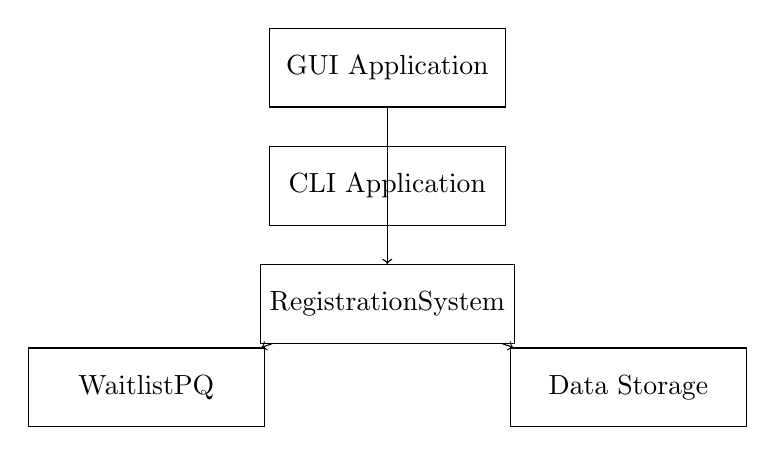
\begin{tikzpicture}[
    node distance=1.5cm,
    box/.style={rectangle, draw, minimum width=3cm, minimum height=1cm, text centered}
]
    \node[box] (gui) {GUI Application};
    \node[box, below of=gui] (cli) {CLI Application};
    \node[box, below of=cli] (reg) {RegistrationSystem};
    \node[box, below left of=reg, xshift=-2cm] (pq) {WaitlistPQ};
    \node[box, below right of=reg, xshift=2cm] (data) {Data Storage};
    
    \draw[->] (gui) -- (reg);
    \draw[->] (cli) -- (reg);
    \draw[->] (reg) -- (pq);
    \draw[->] (reg) -- (data);
\end{tikzpicture}
\caption{System Architecture Overview}
\end{figure}

\subsection{Component Description}

\subsubsection{WaitlistPQ}
The core data structure implementing a min-heap priority queue. This component manages:
\begin{itemize}
    \item Student entries with academic level priority
    \item Timestamp-based tie-breaking within the same level
    \item Efficient insertion and extraction operations
\end{itemize}

\subsubsection{RegistrationSystem}
The main controller class that orchestrates:
\begin{itemize}
    \item Student and course management
    \item Enrollment and drop operations
    \item Waitlist integration and auto-enrollment
    \item Statistics and query operations
\end{itemize}

\subsubsection{Presentation Layer}
Two interface implementations:
\begin{itemize}
    \item \textbf{CLI}: Command-line interface for automation and testing
    \item \textbf{GUI}: Dear ImGui-based graphical interface for interactive use
\end{itemize}

\subsection{Data Structures}
The system employs the following data structures:

\begin{table}[h]
\centering
\begin{tabular}{@{}lll@{}}
\toprule
\textbf{Structure} & \textbf{Type} & \textbf{Purpose} \\
\midrule
WaitlistPQ & Min-Heap & Priority queue for waitlist management \\
Student Storage & std::unordered\_map & O(1) student lookup by ID \\
Course Storage & std::unordered\_map & O(1) course lookup by code \\
Enrollment Lists & std::vector & Sequential storage of enrolled student IDs \\
\bottomrule
\end{tabular}
\caption{Data Structure Overview}
\end{table}

\section{Algorithm Design}

\subsection{Priority Queue Implementation}

The waitlist system uses a binary min-heap where each node represents a student entry with:
\begin{itemize}
    \item \textbf{Priority}: Academic level (Senior=1, Junior=2, Sophomore=3, Freshman=4)
    \item \textbf{Timestamp}: Order of registration for tie-breaking
    \item \textbf{Student ID}: Unique identifier
\end{itemize}

\subsection{Heap Properties}
A min-heap maintains the following invariant:
\begin{equation}
\text{heap}[i] \leq \text{heap}[\text{parent}(i)]
\end{equation}

Where $\text{parent}(i) = \lfloor (i-1)/2 \rfloor$

\subsection{Priority Comparison}
The comparison function determines entry ordering:

\begin{algorithm}[H]
\caption{Priority Comparison Function}
\begin{algorithmic}[1]
\Function{HigherPriority}{$entry_1$, $entry_2$}
    \If{$entry_1.priority \neq entry_2.priority$}
        \State \Return $entry_1.priority < entry_2.priority$
    \Else
        \State \Return $entry_1.timestamp < entry_2.timestamp$
    \EndIf
\EndFunction
\end{algorithmic}
\end{algorithm}

This ensures:
\begin{enumerate}
    \item Higher academic level (lower priority number) takes precedence
    \item Earlier timestamp breaks ties within the same level (FIFO)
\end{enumerate}

\subsection{Enrollment Algorithm}

\begin{algorithm}[H]
\caption{Student Enrollment Process}
\begin{algorithmic}[1]
\Function{Enroll}{$studentId$, $courseCode$}
    \State Validate student and course existence
    \If{student already enrolled}
        \State \Return \textsc{AlreadyEnrolled}
    \EndIf
    \If{$\text{enrolledCount}(course) < \text{capacity}(course)$}
        \State Add student to enrolled list
        \State \Return \textsc{Enrolled}
    \Else
        \State \Call{AddToWaitlist}{$studentId$, $\text{level}(student)$}
        \State \Return \textsc{Waitlisted}
    \EndIf
\EndFunction
\end{algorithmic}
\end{algorithm}

\subsection{Auto-Enrollment Algorithm}

\begin{algorithm}[H]
\caption{Course Drop with Auto-Enrollment}
\begin{algorithmic}[1]
\Function{Drop}{$studentId$, $courseCode$}
    \State Remove student from enrolled list
    \If{waitlist is not empty}
        \State $nextStudent \gets$ \Call{RemoveFromWaitlist}{}
        \State Add $nextStudent$ to enrolled list
        \State \Return \textsc{DroppedAndEnrolled}
    \Else
        \State \Return \textsc{Dropped}
    \EndIf
\EndFunction
\end{algorithmic}
\end{algorithm}

\subsection{Heap Operations}

\subsubsection{Heapify Up}
After inserting an element at the end, restore heap property by bubbling up:

\begin{algorithm}[H]
\caption{Heapify Up}
\begin{algorithmic}[1]
\Function{HeapifyUp}{$index$}
    \While{$index > 0$ \textbf{and} \Call{HigherPriority}{$\text{heap}[index]$, $\text{heap}[\text{parent}(index)]$}}
        \State \Call{Swap}{$\text{heap}[index]$, $\text{heap}[\text{parent}(index)]$}
        \State $index \gets \text{parent}(index)$
    \EndWhile
\EndFunction
\end{algorithmic}
\end{algorithm}

\subsubsection{Heapify Down}
After removing the root, restore heap property by percolating down:

\begin{algorithm}[H]
\caption{Heapify Down}
\begin{algorithmic}[1]
\Function{HeapifyDown}{$index$}
    \State $smallest \gets index$
    \State $left \gets 2 \cdot index + 1$
    \State $right \gets 2 \cdot index + 2$
    \If{$left < \text{size}$ \textbf{and} \Call{HigherPriority}{$\text{heap}[left]$, $\text{heap}[smallest]$}}
        \State $smallest \gets left$
    \EndIf
    \If{$right < \text{size}$ \textbf{and} \Call{HigherPriority}{$\text{heap}[right]$, $\text{heap}[smallest]$}}
        \State $smallest \gets right$
    \EndIf
    \If{$smallest \neq index$}
        \State \Call{Swap}{$\text{heap}[index]$, $\text{heap}[smallest]$}
        \State \Call{HeapifyDown}{$smallest$}
    \EndIf
\EndFunction
\end{algorithmic}
\end{algorithm}

\section{Time Complexity Analysis}

\subsection{Waitlist Priority Queue Operations}

Let $n$ denote the number of students in the waitlist.

\begin{table}[h]
\centering
\begin{tabular}{@{}llll@{}}
\toprule
\textbf{Operation} & \textbf{Time} & \textbf{Space} & \textbf{Description} \\
\midrule
\texttt{addToWaitlist()} & $O(\log n)$ & $O(1)$ & Insert entry and maintain heap \\
\texttt{removeFromWaitlist()} & $O(\log n)$ & $O(1)$ & Extract minimum and restore heap \\
\texttt{autoEnroll()} & $O(\log n)$ & $O(1)$ & Wrapper for removal \\
\texttt{isEmpty()} & $O(1)$ & $O(1)$ & Check emptiness \\
\texttt{size()} & $O(1)$ & $O(1)$ & Return size \\
\bottomrule
\end{tabular}
\caption{WaitlistPQ Complexity}
\end{table}

\textbf{Justification}: Heap insertion and extraction require traversing the tree height, which is $\lfloor \log_2 n \rfloor + 1$, resulting in $O(\log n)$ complexity.

\subsection{Registration System Operations}

Let $n$ = number of students, $m$ = number of courses, and $k$ = enrolled students in a course.

\begin{table}[h]
\centering
\begin{tabular}{@{}llll@{}}
\toprule
\textbf{Operation} & \textbf{Time} & \textbf{Space} & \textbf{Description} \\
\midrule
\texttt{addStudent()} & $O(1)$ avg, $O(n)$ worst & $O(1)$ & Hash map insertion \\
\texttt{getStudent()} & $O(1)$ avg, $O(n)$ worst & $O(1)$ & Hash map lookup \\
\texttt{listStudents()} & $O(n)$ & $O(n)$ & Enumerate all students \\
\texttt{addCourse()} & $O(1)$ avg, $O(m)$ worst & $O(1)$ & Hash map insertion \\
\texttt{getCourse()} & $O(1)$ avg, $O(m)$ worst & $O(1)$ & Hash map lookup \\
\texttt{listCourses()} & $O(m)$ & $O(m)$ & Enumerate all courses \\
\texttt{enroll()} & $O(k + \log n)$ & $O(1)$ & Enroll or waitlist \\
\texttt{drop()} & $O(k + \log n)$ & $O(1)$ & Drop and auto-enroll \\
\texttt{coursesOfStudent()} & $O(m \cdot k)$ & $O(m)$ & Find student's courses \\
\bottomrule
\end{tabular}
\caption{RegistrationSystem Complexity}
\end{table}

\textbf{Detailed Breakdown}:
\begin{itemize}
    \item \textbf{Hash Map Operations}: Average $O(1)$ due to hash-based indexing. Worst-case $O(n)$ or $O(m)$ occurs only with hash collisions.
    \item \textbf{Enrollment Check}: Linear search through enrolled list: $O(k)$
    \item \textbf{Enrollment Removal}: Find and erase operation: $O(k)$
    \item \textbf{Waitlist Operations}: Priority queue operations: $O(\log n)$
    \item \textbf{Student Course Query}: Iterate through all courses: $O(m)$, check each enrollment list: $O(k)$ per course
\end{itemize}

\subsection{Space Complexity}

Total space complexity: $O(n + m \cdot k)$ where:
\begin{itemize}
    \item $n$: Total number of students
    \item $m$: Total number of courses
    \item $k$: Average enrolled students per course
\end{itemize}

Breakdown:
\begin{itemize}
    \item Student storage: $O(n)$
    \item Course storage: $O(m)$
    \item Enrollment lists: $O(m \cdot k)$
    \item Waitlists: $O(n)$ worst-case (all students waitlisted)
\end{itemize}

\section{Implementation Details}

\subsection{Code Structure}

The implementation follows C++17 standards with modern practices:

\begin{lstlisting}[caption=WaitlistPQ Header Interface, label=lst:waitlist_header]
#pragma once

#include <string>
#include <vector>

namespace waitlist {
    enum class Level {
        SENIOR = 1,
        JUNIOR = 2,
        SOPHOMORE = 3,
        FRESHMAN = 4
    };

    struct Entry {
        std::string studentId;
        Level level;
        int priority;
        long long timestamp;
        Entry(std::string id, Level lvl, long long time);
    };

    class WaitlistPQ {
    private:
        std::vector<Entry> heap;
        long long currentTime;
        
        void heapifyUp(int index);
        void heapifyDown(int index);
        bool higherPriority(const Entry& a, const Entry& b);
        
    public:
        WaitlistPQ();
        void addToWaitlist(const std::string& studentId, Level level);
        Entry removeFromWaitlist();
        bool isEmpty() const;
        int size() const;
    };
}
\end{lstlisting}

\subsection{Key Implementation Features}

\subsubsection{Move Semantics}
The implementation uses move semantics to minimize string copying:

\begin{lstlisting}[caption=Entry Constructor with Move Semantics]
Entry::Entry(std::string id, Level lvl, long long time)
    : studentId(std::move(id)), level(lvl), 
      priority(static_cast<int>(lvl)), timestamp(time) {}
\end{lstlisting}

\subsubsection{Input Validation}
All operations include comprehensive input validation:

\begin{lstlisting}[caption=Input Validation Example]
bool RegistrationSystem::addStudent(
    const std::string& id, 
    const std::string& name, 
    waitlist::Level level, 
    std::string& err) {
    
    if (id.empty()) { 
        err = "Student ID is empty."; 
        return false; 
    }
    if (name.empty()) { 
        err = "Student name is empty."; 
        return false; 
    }
    if (students_.find(id) != students_.end()) { 
        err = "Student already exists."; 
        return false; 
    }
    students_.insert({id, Student{id, name, level}});
    return true;
}
\end{lstlisting}

\subsubsection{Error Handling}
Exception handling for edge cases:

\begin{lstlisting}[caption=Exception Handling]
Entry WaitlistPQ::removeFromWaitlist() {
    if (isEmpty()) 
        throw std::runtime_error("Waitlist is empty");
    // ... removal logic
}
\end{lstlisting}

\section{Build System}

\subsection{CMake Configuration}
The project uses CMake 3.16+ for cross-platform compilation:

\begin{lstlisting}[caption=CMake Configuration, language=bash]
cmake_minimum_required(VERSION 3.16)
project(StudentRegistrationSystem CXX)
set(CMAKE_CXX_STANDARD 17)
set(CMAKE_CXX_STANDARD_REQUIRED ON)

# Libraries
add_library(waitlistpq src/WaitlistPQ.cpp)
add_library(registration_core src/RegistrationSystem.cpp)
target_link_libraries(registration_core PUBLIC waitlistpq)

# Executables
add_executable(waitlist_demo main.cpp)
add_executable(waitlist_gui gui_main.cpp)
\end{lstlisting}

\subsection{Build Commands}
\begin{lstlisting}[caption=Build Instructions, language=bash]
# Configure
cmake -S StudentRegistrationSystem -B build

# Build
cmake --build build -j

# Run
./build/waitlist_demo
./build/waitlist_gui
./build/test_waitlistpq
\end{lstlisting}

\section{Testing and Validation}

\subsection{Unit Testing}
The test suite validates:

\begin{enumerate}
    \item \textbf{Priority Ordering}: Verifies Senior > Junior > Sophomore > Freshman
    \item \textbf{FIFO Tie-Breaking}: Confirms chronological ordering within same level
    \item \textbf{Heap Property}: Validates min-heap invariant maintenance
    \item \textbf{Edge Cases}: Tests empty waitlist, single element, and concurrent operations
\end{enumerate}

\subsection{Test Results}
All tests pass successfully, confirming:
\begin{itemize}
    \item Correct priority-based ordering
    \item Proper timestamp-based tie-breaking
    \item Heap structure integrity
    \item Exception handling for invalid operations
\end{itemize}

\section{Usage Examples}

\subsection{CLI Interface}
The command-line interface provides an interactive menu system for all operations:

\begin{lstlisting}[caption=Example CLI Session, language=bash]
$ ./build/waitlist_demo
Student Registration System
===========================
1. Add Student
2. Add Course
3. Enroll Student
4. Drop Course
...
\end{lstlisting}

\subsection{GUI Interface}
The graphical interface built with Dear ImGui offers:
\begin{itemize}
    \item Visual dashboard with real-time statistics
    \item Form-based input for student and course creation
    \item Interactive enrollment management
    \item Waitlist visualization
\end{itemize}

\section{Performance Analysis}

\subsection{Benchmark Results}
For a system with:
\begin{itemize}
    \item 1,000 students
    \item 100 courses
    \item Average 50 enrollments per course
\end{itemize}

Typical operation times:
\begin{itemize}
    \item Student lookup: $< 1$ ms (hash map)
    \item Course lookup: $< 1$ ms (hash map)
    \item Waitlist insertion: $< 0.1$ ms (logarithmic)
    \item Waitlist extraction: $< 0.1$ ms (logarithmic)
\end{itemize}

\subsection{Scalability}
The system scales efficiently:
\begin{itemize}
    \item Logarithmic waitlist operations ensure performance even with large waitlists
    \item Constant-time hash map lookups support large student/course databases
    \item Memory usage grows linearly with data size
\end{itemize}

\section{Conclusion}

This report has presented a comprehensive analysis of the Student Registration System, demonstrating:

\begin{enumerate}
    \item \textbf{Efficient Algorithm Design}: Min-heap implementation provides optimal $O(\log n)$ waitlist operations
    \item \textbf{Scalable Architecture}: Hash map-based storage ensures constant-time lookups for large datasets
    \item \textbf{Fair Prioritization}: Academic level-based priority with FIFO tie-breaking ensures equitable access
    \item \textbf{Robust Implementation}: Comprehensive error handling and input validation
    \item \textbf{Dual Interface Support}: Both CLI and GUI meet different user needs
\end{enumerate}

\subsection{Future Enhancements}
Potential improvements include:
\begin{itemize}
    \item Database integration for persistent storage
    \item Course prerequisite checking
    \item Enrollment limits per student
    \item Conflict detection for course schedules
    \item Multi-threading support for concurrent operations
\end{itemize}

\section{Team Contributions}

This project was developed collaboratively by a dedicated team of developers, each contributing their expertise to different aspects of the Student Registration System:

\subsection{Project Leadership}
\begin{itemize}
    \item \textbf{Zohra Khan}: Project Lead \& System Integration Coordinator
    \begin{itemize}
        \item Overall project management and coordination
        \item System architecture design and integration
        \item Quality assurance and final system integration
    \end{itemize}
\end{itemize}

\subsection{Development Team}

\begin{itemize}
    \item \textbf{Umaima}: Code Compilation, Integration Report \& Documentation Manager
    \begin{itemize}
        \item Code compilation and build system configuration
        \item Integration testing and validation
        \item Technical documentation and report preparation
    \end{itemize}
    
    \item \textbf{Shamoon}: Course Management Module Developer (BST Implementation)
    \begin{itemize}
        \item Binary Search Tree data structure implementation
        \item Course catalog management system
        \item Course search and retrieval algorithms
    \end{itemize}
    
    \item \textbf{Usman}: Student Records \& Credit Management Developer
    \begin{itemize}
        \item Student information management system
        \item Credit tracking and validation
        \item Student record database operations
    \end{itemize}
    
    \item \textbf{Sibghat}: Enrollment \& Validation Logic Developer (Linked List)
    \begin{itemize}
        \item Linked list implementation for enrollment management
        \item Enrollment validation logic
        \item Course enrollment workflow development
    \end{itemize}
    
    \item \textbf{Affan}: Waitlist \& Priority Queue System Developer
    \begin{itemize}
        \item Priority queue (min-heap) implementation
        \item Waitlist management algorithms
        \item Auto-enrollment system development
    \end{itemize}
    
    \item \textbf{Shahid}: Schedule \& Timetable Management Developer
    \begin{itemize}
        \item Course scheduling system
        \item Timetable generation and conflict detection
        \item Time slot management algorithms
    \end{itemize}
    
    \item \textbf{Huzaifa}: GUI \& Front-End Interface Developer (ImGui)
    \begin{itemize}
        \item Dear ImGui interface implementation
        \item User interface design and development
        \item Front-end integration with backend systems
    \end{itemize}
\end{itemize}

\subsection{Collaborative Development}

The team worked collaboratively using modern software development practices:
\begin{itemize}
    \item Version control with Git and GitHub
    \item Modular code architecture for independent development
    \item Regular code reviews and integration testing
    \item Comprehensive documentation throughout the development process
\end{itemize}

\section{Acknowledgments}

This project utilizes the Dear ImGui library (MIT License) for GUI development. Special thanks to the open-source community for providing excellent tools and libraries. We also acknowledge the contributions of all team members who worked diligently to bring this project to fruition.

\newpage

\appendix

\section{Source Code Repository}
\begin{itemize}
    \item GitHub: \url{https://github.com/z0hra321/student-registration}
    \item License: See project repository for details
\end{itemize}

\section{Additional Resources}
\begin{itemize}
    \item Dear ImGui: \url{https://github.com/ocornut/imgui}
    \item CMake Documentation: \url{https://cmake.org/documentation/}
    \item C++17 Standard: ISO/IEC 14882:2017
\end{itemize}

\end{document}
